\documentclass{article}
% Package setup
% To use < and >... Yes...
\usepackage[T1]{fontenc}

% UML diagrams
\usepackage{tikz-uml}

% Floats
\usepackage{float}

% Captions
\usepackage[labelfont=bf]{caption}

% HyperRef
\usepackage{color}   %May be necessary if you want to color links
\usepackage{hyperref}
\hypersetup{
    colorlinks=true, %set true if you want colored links
    linktoc=all,
    linkcolor=black,
    urlcolor=blue
}

% Code listings
\usepackage{listings}
\usepackage{textcomp}

% Scheme style definition
\lstdefinelanguage{Scheme}{
  morekeywords=[1]{define, define-syntax, define-macro, lambda, define-stream, stream-lambda},
  morekeywords=[2]{begin, call-with-current-continuation, call/cc,
    call-with-input-file, call-with-output-file, case, cond,
    do, else, for-each, if,
    let*, let, let-syntax, letrec, letrec-syntax,
    let-values, let*-values,
    and, or, not, delay, force,
    quasiquote, quote, unquote, unquote-splicing,
    map, fold, syntax, syntax-rules, eval, environment, query, nil },
  morekeywords=[3]{import, export},
  alsodigit=!\$\%&*+-./:<=>?@^_~,
  sensitive=true,
  morecomment=[l]{;},
  morecomment=[s]{\#|}{|\#},
  morestring=[b]",
  basicstyle=\small\ttfamily,
  keywordstyle=\bf\ttfamily\color[rgb]{0,.3,.7},
  commentstyle=\color[rgb]{0.133,0.545,0.133},
  stringstyle={\color[rgb]{0.75,0.49,0.07}},
  upquote=true,
  breaklines=true,
  breakatwhitespace=true,
  literate=*{`}{{`}}{1},
  tabsize=2
}

\begin{document}
% Top matter
\title{CGEN LLVM-IR \\ Design Document \vfill}
\author{Leonardo Arcari \\ Politecnico di Milano}
\date{February 2018}
\maketitle
\thispagestyle{empty}
\clearpage

% Table of contents
\tableofcontents
\clearpage

% Introductory section
\pagenumbering{arabic}
\section{Introduction}
\subsection{Scope}
This document is meant to provide a resource to those who are going to work with GNU CGEN and my extension to it: CGEN LLVM-IR. The purpose of this paper is to introduce the reader first to GNU CGEN from a code perspective, as GNU CGEN already provides a user guide. The reader will find in this document a code analysis, with a, possibly more clear, description of the main classes in Scheme source code in order to use them effectively.

In second place, I will provide a similar description of the code that I wrote in order to extend GNU CGEN to allow the generation of C++ programs capable of translating binary programs into a semantically equivalent representation in LLVM-IR language.

\subsection{Out of scope}
In this paper I am not going to describe several topics related to GNU CGEN
\begin{itemize}
\item How to run GNU CGEN. There is a manual online for it.\footnote{\url{https://sourceware.org/cgen/docs/cgen_2.html}}
\item What is the plethora of features of GNU CGEN. There is a manual online for it.\footnote{\url{https://sourceware.org/cgen/docs/cgen_1.html}}
\item What is CGEN RTL and what each language feature does. There is a manual online for it.\footnote{\url{https://sourceware.org/cgen/docs/cgen_3.html}}
\item How to write a CGEN application to define your CPU architecture in RTL. Guess what? There's a manual online for it.\footnote{\url{https://sourceware.org/cgen/docs/cgen_8.html}}
\end{itemize}
Also, a pre-requisite to understand completely this document, the reader should know Lisp in one of its dialects. For soundness, be aware that CGEN is written in Scheme in the dialect implemented by Guile 1.8.0.

\subsection{Project History}
CGEN LLVM-IR generator is part of the project I was assigned to while taking the \emph{Code Transformation and Optimization} course held by Professor G. Agosta\footnote{\url{https://home.deib.polimi.it/agosta}} in the A.Y. 2017/2018. The idea of extending GNU CGEN, in order to generate C++ translators capable of producing a semantically-equivalent representation in LLVM-IR of a binary for a given architecture, is from Alessandro Di Federico, PhD\footnote{\url{https://clearmind.me/}}. 

\clearpage
\section{GNU CGEN}
\subsection{Introduction to CGEN}
In this section I would like to give a high-level presentation of GNU CGEN, what it is useful for and why we think that provides enough value for the purposes of our project.
\paragraph{Goal}
``The goal of CGEN (pronounced seejen, and short for "Cpu tools GENerator") is to provide a uniform framework and toolkit for writing programs like assemblers, disassemblers, and simulators without explicitly closing any doors on future things one might wish to do. In the end, its scope is the things the software developer cares about when writing software for the cpu (compilation, assembly, linking, simulation, profiling, debugging, ???)''\footnote{\url{https://sourceware.org/cgen/docs/cgen_1.html\#SEC3}}.

They way CGEN plans to achieve this goal is centered around having a CPU description language, called \emph{RTL}, totally agnostic about the final goal. In RTL the programmer can describe:
\begin{description}
\item [CPU architectures] General purpose registers, status registers
\item [ISA] Instructions, operands, instruction formats, instruction fields
\item [Semantics] What is the output, what registers change and how when instruction A is executed?
\end{description}

And a lot more\footnote{\url{https://sourceware.org/cgen/docs/cgen_3.html}}.

\paragraph{Project idea}
The idea behind our project, CGEN LLVM-IR, is the following. CGEN is already able to generate GDB simulators for any architecture given its description in RTL language. Simulators, very simplistically, accept a binary program as input, emulate the hardware architecture in memory by means of variables to represent registers and emulate the execution of the input program line of code by line of code. This looks a lot like our objective.

If we were required to outline the execution of our project, in fact, that would by sketched by the following steps:
\begin{itemize}
\item Allocate a set of LLVM-IR global variables to mock general purpose registers, program counter and CPU status registers.
\item Disassemble the binary input to reconstruct the assembly instructions and their operands.
\item Through LLVM framework, emit LLVM-IR code that mimics the semantic of each istruction and sets our \emph{mock registers} correctly.
\end{itemize}

With this workflow in mind, our approach was as much as conservative as we could. We wanted to reuse CGEN code as much as possible, so we analyzed CGEN source code deeply. We started by looking at the those components that were responsible of generating the GDB simulator.

We discovered that the frontend part of CGEN could be easily reused. Frontend components tackles the problem of parsing RTL language to build an internal representation of language constructs and access their data efficiently.

So language parsing and data structures were there to be used. We could not say the same for components dealing with simulators generation.

It should be noted that GDB simulators are C programs, so CGEN was coded to emit C lines of code. Those components would have been a great reference for the logic that drives disassembling and instruction simulation, but they were required to be completely rewritten to emit C++ code. Unfortunately the C code generation was so tightly coupled in them that we had to write a whole new set of components to address our needs. More details are provided in section \ref{sec:cgen-llvm-ir}.
\clearpage

\subsection{CGEN RTL classes}
In this part of the document I want to provide an insight of Scheme classes in CGEN that represent internally the language constructs of RTL and allow the programmer to access the data written in the CPU description file.

To better understand the relationship between classes, I first present an example of the structure of an RTL description.

\begin{figure}[H]
	\centering
	\begin{tikzpicture}
		\umlsimpleclass[x=0, y=0]{Architecture}
		\umlsimpleclass[x=-2.5, y=-1]{cpu-family1}
		\umlsimpleclass[x=-4, y=-2]{machine1}
		\umlsimpleclass[x=-1, y=-2]{machine2}
		\umlsimpleclass[x=2.5, y=-1]{cpu-family2}
		\umlsimpleclass[x=4, y=-2]{machine3}
		
		\umlassoc{Architecture}{cpu-family1}
		\umlassoc{Architecture}{cpu-family2}
		\umlassoc{cpu-family1}{machine1}
		\umlassoc{cpu-family1}{machine2}
		\umlassoc{cpu-family2}{machine3}
	\end{tikzpicture}
	\caption{A graphical layout of top level RTL elements. The architecture is one of `sparc', `m32r', etc. Within the `sparc' architecture, cpu-family might be `sparc32', `sparc64', etc. Within the `sparc32' CPU family, the machine might be `sparc-v8', `sparclite', etc.}
\end{figure}

\begin{figure}[H]
	\centering
	\begin{tikzpicture}
		\umlsimpleclass[x=0, y=0]{ISA}
		\umlsimpleclass[x=0, y=-1]{Instruction}
		\umlsimpleclass[x=-2, y=-2]{operand1}
		\umlsimpleclass[x=2, y=-2]{operand2}
		\umlsimpleclass[x=-2, y=-3]{hw1+ifield1}
		\umlsimpleclass[x=2, y=-3]{hw2+ifield2}
		
		\umlassoc{ISA}{Instruction}
		\umlassoc{Instruction}{operand1}
		\umlassoc{Instruction}{operand2}
		\umlassoc{operand1}{hw1+ifield1}
		\umlassoc{operand2}{hw2+ifield2}
	\end{tikzpicture}
	\caption{Instructions form their own hierarchy as each instruction may be supported by more than one machine}
\end{figure}

\subsubsection{CGEN's object system - cos.scm}
Although Guile, the Scheme implementation supported by CGEN, provided an official object system in the 1.8 release, the CGEN author thought that things might have changed and he wanted to be sure not to be required to change the entire CGEN code base in case that happened. Thus he decided to implement his own object system and we must deal with it. I'm going to give a presentation of those feature that you might come across while working on CGEN codebase and you might need to know.

\paragraph{Class}
Classes is CGEN are implemented (of course) as vectors of information defining your class, as you can see in listing \ref{lst:class}
\lstset{
	frame=single,
	numbers=left,
	upquote=true
}
\begin{figure}[H]
\begin{lstlisting}[language=Scheme, label=lst:class, caption=A class in CGEN looks like this]
#(class-tag
	class-name
	parent-name-list
	elm-alist
	method-alist
	full-elm-initial-list
	class-descriptor)
\end{lstlisting}
\end{figure}

The fields you should care about are the following:
\begin{description}
\item[class-name] A name uniquely defining the class. E.g: \texttt{<arch>}
\item[parent-name-list] A list of the names of parent classes (the inheritance tree).
\item[elm-alist] A list of \texttt{(symbol private? vector-index . initial-value)} for this class only.
\item[method-alist] An alist of \texttt{(symbol . (virtual? . procedure))} for this class only.
\end{description}

To declare a new class: \texttt{(class-make name parents elements methods)}
An example of class declaration is available at listing \ref{lst:class-decl}

\begin{figure}[H]
\begin{lstlisting}[language=Scheme, label=lst:class-decl, caption=An example of class declaration in CGEN]
(define <mach>
	(class-make 
		'<mach>
		'(<ident>)
		'(
			; cpu family this mach is a member of
			cpu
			; bfd name of mach
			bfd-name
			; list of <isa> objects
			isas
		)
		nil)
)
\end{lstlisting}
\end{figure}

The above example shows a common practice in CGEN. Methods are defined after class declaration with the help of some macros/procedures.

\paragraph{Getters and Setters declaration}
To add getters and setters method to a class two convenient macros are provided:\\
\texttt{define-getters (class class-prefix elm-names)} \\
\texttt{define-setters (class class-prefix elm-names)}


\paragraph{Other methods declaration}
For all other kinds of methods two procedures are available:\\
\texttt{(method-make! class name lambda)} \\
\texttt{(method-make-virtual! class name lambda)}

\begin{figure}[H]
\begin{lstlisting}[language=Scheme, caption=Example of methods declaration for a class]
; Define getters for class <mach> for members
; 'cpu', 'bfd-name' and 'isas' and name them
; 'mach-<member>' where <member> is
; [cpu|bfd-name|isas]
(define-getters <mach> mach (cpu bfd-name isas))

; Define setter for class <ifield> for member
; 'follows' and name it 'ifld-follows'
(define-setters <ifield> ifld (follows))

; Define a method for class <ifield> named
; 'get-field-value whose implementation is
; defined by the lambda
(method-make!
 <ifield> 'get-field-value
 (lambda (self)
   (elm-get self 'value))
)
\end{lstlisting}
\end{figure}

\paragraph{Method invokation}
CGEN's object system follows the Smalltalk way of implementing object orientation, that is by means of \emph{messages}. Thus we can invoke a method on  an object with:\\
\texttt{(send object method-name . args)}

\begin{figure}[H]
\begin{lstlisting}[language=Scheme, caption=Example of methods invokation]
; We wrap a method invokation in a standard
; Scheme procedure for simplicity of usage
(define (ifld-set-value! self new-val)
  (send self 'set-field-value! new-val)
)
\end{lstlisting}
\end{figure}

\subsubsection{Arch - mach.scm}
Arch is the top level class in CGEN that records everything about a CPU.
After parsing a .cpu file the programmer can refer to a global variable named \texttt{CURRENT-ARCH} to access an instance of Arch.

\begin{figure}[H]
	\centering
	\begin{tikzpicture}
		\umlclass[x=0, y=0, name=Arch]{Arch}{
			+ default-alignment : [aligned|unaligned|forced] \\
			+ insn-lsb0? : bool \\
			+ machs : (mach-name . sanitize-key)* \\
			+ isas : (isa-name . sanitize-key)*
		}{
			+ current-arch-name () $\rightarrow$ str? \\
			+ current-arch-insn-lsb0? () $\rightarrow$ boolean? \\
			+ current-cpu-list () $\rightarrow$ list?\\
			+ \ldots
		}
		\umlsimpleclass[x=-3.5, y=4]{Attribute}
		\umlsimpleclass[x=-1.25, y=4]{Enum}
		\umlsimpleclass[x=1, y=4]{Hardware}
		\umlsimpleclass[x=3.5, y=4]{Keyword}
		\umlsimpleclass[x=-3.5, y=-4]{Isa}
		\umlsimpleclass[x=3.5, y=-4]{Mach}
		\umlsimpleclass[x=-1.5, y=-4]{Insn}
		\umlsimpleclass[x=1.5, y=-4]{Sfmt}
		
		\umlunicompo[mult=1..*, pos2=0.6]{Arch}{Attribute}
		\umlunicompo[mult=1..*, pos2=0.6]{Arch}{Enum}
		\umlunicompo[mult=1..*]{Arch}{Hardware}
		\umlunicompo[mult=1..*]{Arch}{Keyword}
		\umlunicompo[mult=1..*]{Arch}{Isa}
		\umlunicompo[mult=1..*, pos2=0.55]{Arch}{Mach}
		\umlunicompo[mult=1..*]{Arch}{Insn}
		\umlunicompo[mult=1..*, pos2=0.6]{Arch}{Sfmt}
	\end{tikzpicture}
	\caption{Class diagram of <arch> CGEN class}
\end{figure}

\subsubsection{Hardware - hardware.scm}
\texttt{<hardware-base>} is the base class for all hardware descriptions. The actual hardware objects inherit from this (e.g. register, immediate). This is used to describe registers, memory, and immediates.

\texttt{mode} in diagram \ref{fig:hw-base} refers to one of the many data types you can specify in RTL. \href{https://sourceware.org/cgen/docs/cgen_3.html\#SEC161}{Look here for more information}.

\begin{figure}[H]
	\centering
	\begin{tikzpicture}
		\umlclass[x=0, y=0, name=<hardware-base>]{<hardware-base>}{
			+ sem-name : str?
		}{
			+ \ldots
		}
		\umlclass[x=2.5, y=2.25, name=<hw-asm>]{<hw-asm>}{
			mode : [VOID|UINT|\ldots]	
		}{}
		\umlclass[x=-2.5, y=3, name=<array>]{<array>}{
			+ mode : [VOID|UINT|\ldots] \\
			+ dimensions : list?
		}{
			+ get-mode() $\rightarrow$ atom? \\
			+ get-rank() $\rightarrow$ number? \\
			+ get-shape() $\rightarrow$ list?
		}
		\umlsimpleclass[x=-1.5, y=-2]{<hw-register>}
		\umlsimpleclass[x=1.5, y=-2]{<hw-pc>}

		
		\umlunicompo[geometry=-|, mult=1..*, pos2=1.8]{<hardware-base>}{<hw-asm>}
		\umlunicompo[geometry=-|, mult=1..*, pos2=1.8]{<hardware-base>}{<array>}
		\umlinherit{<hw-register>}{<hardware-base>}
		\umlinherit{<hw-pc>}{<hardware-base>}
	\end{tikzpicture}
	\caption{Class diagram of hardware.scm CGEN classes}
	\label{fig:hw-base}
\end{figure}

\subsubsection{Instruction - insn.scm}
\texttt{<insn>} is the class to hold an instruction. This class is very important as it is an entry point to deal with instruction disassembling and translating into LLVM-IR.

The programmer can retrieve the parsed list of ISA instructions with the nullary procedure \texttt{current-insn-list}.

\texttt{semantics} member of \texttt{<insn>} contains the RTL source code explaining the instruction semantic. This gets compiled by CGEN and transformed into an \texttt{<rtx-func>} object representing the RTL expression in Scheme. The \texttt{<rtx-func>} object is stored in \texttt{compiled-semantics} member.

\texttt{bitrange} member of \texttt{<ifield>} contains the field's offset, start, length, word-length and orientation ($msb==0$, $lsb==0$). Although this seems promising data, it is \emph{not trustworthy}. In fact, current stable release of CGEN (1.1 at the moment of writing) has issues in dealing with ISAs with variable length instructions, thus some values like \texttt{length} or \texttt{word-length} might be wrong. According to my research on this topic, only ISAs with instruction of fixed length (say 32bit) allow the programmer to exploit and trust values within \texttt{bitrange} member. For more complex architectures that value is misleading so it should be ignored.
Some \emph{.cpu} declaring weird istruction sets provided a custom way to fetch instructions from binary programs. This requires more investigation.

\begin{figure}[H]
	\centering
	\begin{tikzpicture}
		\umlclass[x=0, y=0, name=<insn>]{<insn>}{
			+ syntax : str? \\
			+ semantics : str? \\
			+ compiled-semantics : <rtx-func>?
		}{
			+ \ldots
		}
		\umlclass[x=4, y=-3.5, name=<ifield>]{<ifield>}{
			mode : [VOID|UINT|\ldots] \\
			bitrange: <bitrange>? \\
		}{}
		\umlclass[x=-2.5, y=-3.5, name=<array>]{<iformat>}{
			+ mask-length : integer? \\
			+ length : integer? \\
			+ mask : integer?
		}{}
		\umlclass[x=-2.5, y=-6, name=<sformat>]{<sformat>}{
			+ length : integer? \\		
		}{}
		\umlunicompo[geometry=-|, mult=1..*, pos2=1.9]{<insn>}{<ifield>}
		\umlunicompo[geometry=-|, mult=1..*, pos2=1.7]{<sformat>}{<ifield>}
		\umlunicompo[mult=1..*]{<iformat>}{<ifield>}
		\umlunicompo[mult=1]{<insn>}{<iformat>}
		\umlunicompo[geometry=|-, anchors=-80 and 10, mult=1, pos2=1.8]{<insn>}{<sformat>}
	\end{tikzpicture}
	\caption{Class diagram of insn.scm and iformat.scm CGEN classes}
\end{figure}

\subsubsection{Ident - a common base class}
One thing I did not mention so far is that every class described in this section inherits from a general base class: \texttt{<ident>}.

\begin{figure}[H]
\begin{lstlisting}[language=Scheme, caption=<ident> class declaration]
(define <ident>
	(class-make '<ident> '()
		'(name comment attrs)
		'()))

; getters and setters...
\end{lstlisting}
\end{figure}

\begin{description}
\item[name] Names must be valid Scheme symbols.
\item[comment] Comments may be any number of lines, though generally succinct comments are preferable.
\item[attributes] A list of attributes\footnote{\url{https://sourceware.org/cgen/docs/cgen_3.html\#SEC56}}
\end{description}
\clearpage

\subsection{Code Analysis}
\subsubsection{Entry Point}
\subsubsection{RTL-C Generator}

\clearpage
\section{CGEN LLVM-IR} \label{sec:cgen-llvm-ir}
\subsection{CGEN-IR common}
\subsection{IR-Gen registers}
\subsection{IR-Gen decoder}
\subsection{RTL-CPP Generator}
\end{document}
